\documentclass[letter]{bioinfo}
\copyrightyear{2018} \pubyear{2018}
\usepackage{soul} %highlight stuff

%bibliography magic
\usepackage{natbib}
\setlength{\bibsep}{\baselineskip} %dbl space between citations

\usepackage{hyperref}
\access{Advance Access Publication Date: (under review)}
\appnotes{Review article}
\graphicspath{{../figures/}}

\newcommand{\comment}[1]{\textcolor{red}{#1}}
\newcommand{\todo}[1]{\colorbox{yellow}{\parbox{1\linewidth}{#1}}}


\begin{document}
	\firstpage{1}
	
	\subtitle{Review}
	
	\title[Cardioinformatics]{Cardioinformatics: the nexus of bioinformatics and cardiology}
	\author[Khomtchouk \textit{et~al}.]{Bohdan B. Khomtchouk\,$^{\text{\sfb 1,2,3,}*,$\dag$}$,\, Diem-Trang Tran\,$^{\text{\sfb 4},$\dag$}$, Or Gozani\,$^{\text{\sfb 1}}$, Matthew Might\,$^{\text{\sfb 5}}$, Themistocles L. Assimes\,$^{\text{\sfb 2, 3}}$}
	\address{$^{\text{\sf 1}}$Department of Biology, Stanford University, Stanford, CA, USA \\
		$^{\text{\sf 2}}$Department of Medicine, Division of Cardiovascular Medicine, Stanford University, Stanford, CA, USA \\
		$^{\text{\sf 3}}$VA Palo Alto Health Care System, Palo Alto, CA, USA \\
		$^{\text{\sf 4}}$School of Computing, University of Utah, Salt Lake City, UT, USA \\
		$^{\text{\sf 5}}$Hugh Kaul Personalized Medicine Institute, University of Alabama at Birmingham, Birmingham, AL, USA \\
	}
	
	\corresp{$^\ast$To whom correspondence should be addressed: \href{bohdan@stanford.edu}{bohdan@stanford.edu}\\
	$^\dagger$These authors contributed equally to this work.
	}

	
	\history{Received on XXXXX; revised on XXXXX; accepted on XXXXX}
	
	\editor{Associate Editor: XXXXXXX}
	
	\abstract{Cardiovascular disease (CVD) is the leading cause of death worldwide, causing over 17M deaths per year, which outpaces global cancer mortality rates.  Despite these sobering statistics, most bioinformatics and computational biology work to-date has been concentrated predominantly on cancer research, with a relatively modest footprint in CVD.  In this paper, we review the existing literary landscape and critically assess the unmet need to pioneer an emerging field at the multidisciplinary interface of bioinformatics and cardiology, which we refer to as "cardioinformatics".  To promote reproducibility, all data and source code powering the data-driven visualizations and quantitative analyses presented in this review are provided at: https://github.com/Bohdan-Khomtchouk/cardioinformatics. \\
		\textbf{Keywords:} cardiovascular disease; bioinformatics; cardiology; computational biology}
	
\maketitle
	
\section*{Introduction}
	%\section*{The current status of bioinformatics in cardiovascular disease research}
	
Cardiovascular diseases have persistently been the leading cause of death by non-communicable diseases in the US for the last two decades (Figure \ref{fig:figure1}A).  According to the World Health Organization, ischemic heart disease and stroke have remained the top two global killers in the last 15 years, with cancer (all cancers combined) currently ranked number three.  The Global Burden of Diseases, Injuries, and Risk Factors Study shows that while heart disease and cancer have similar mortality rates in the US, heart disease is still the dominant cause of death globally for both genders \citep{Roth:2018:Global}.  Research in CVD has steadily increased since the year 2000, as measured by the body of publications indexed in PubMed over this time (Figure \ref{fig:figure1}B).  In 2017 alone, there were more than 40000 primary research (non-review) articles classified with the subject heading "cardiovascular disease", defined according to the Medical Subject Heading (MeSH) terms.  This MeSH Database entry (\textit{cardiovascular disease}) includes many types of cardiovascular abnormalities that may occur in organs outside the immediate circulatory system, highlighting the complex disease nature of CVD.


\begin{figure}[!tpb]
	\centering
	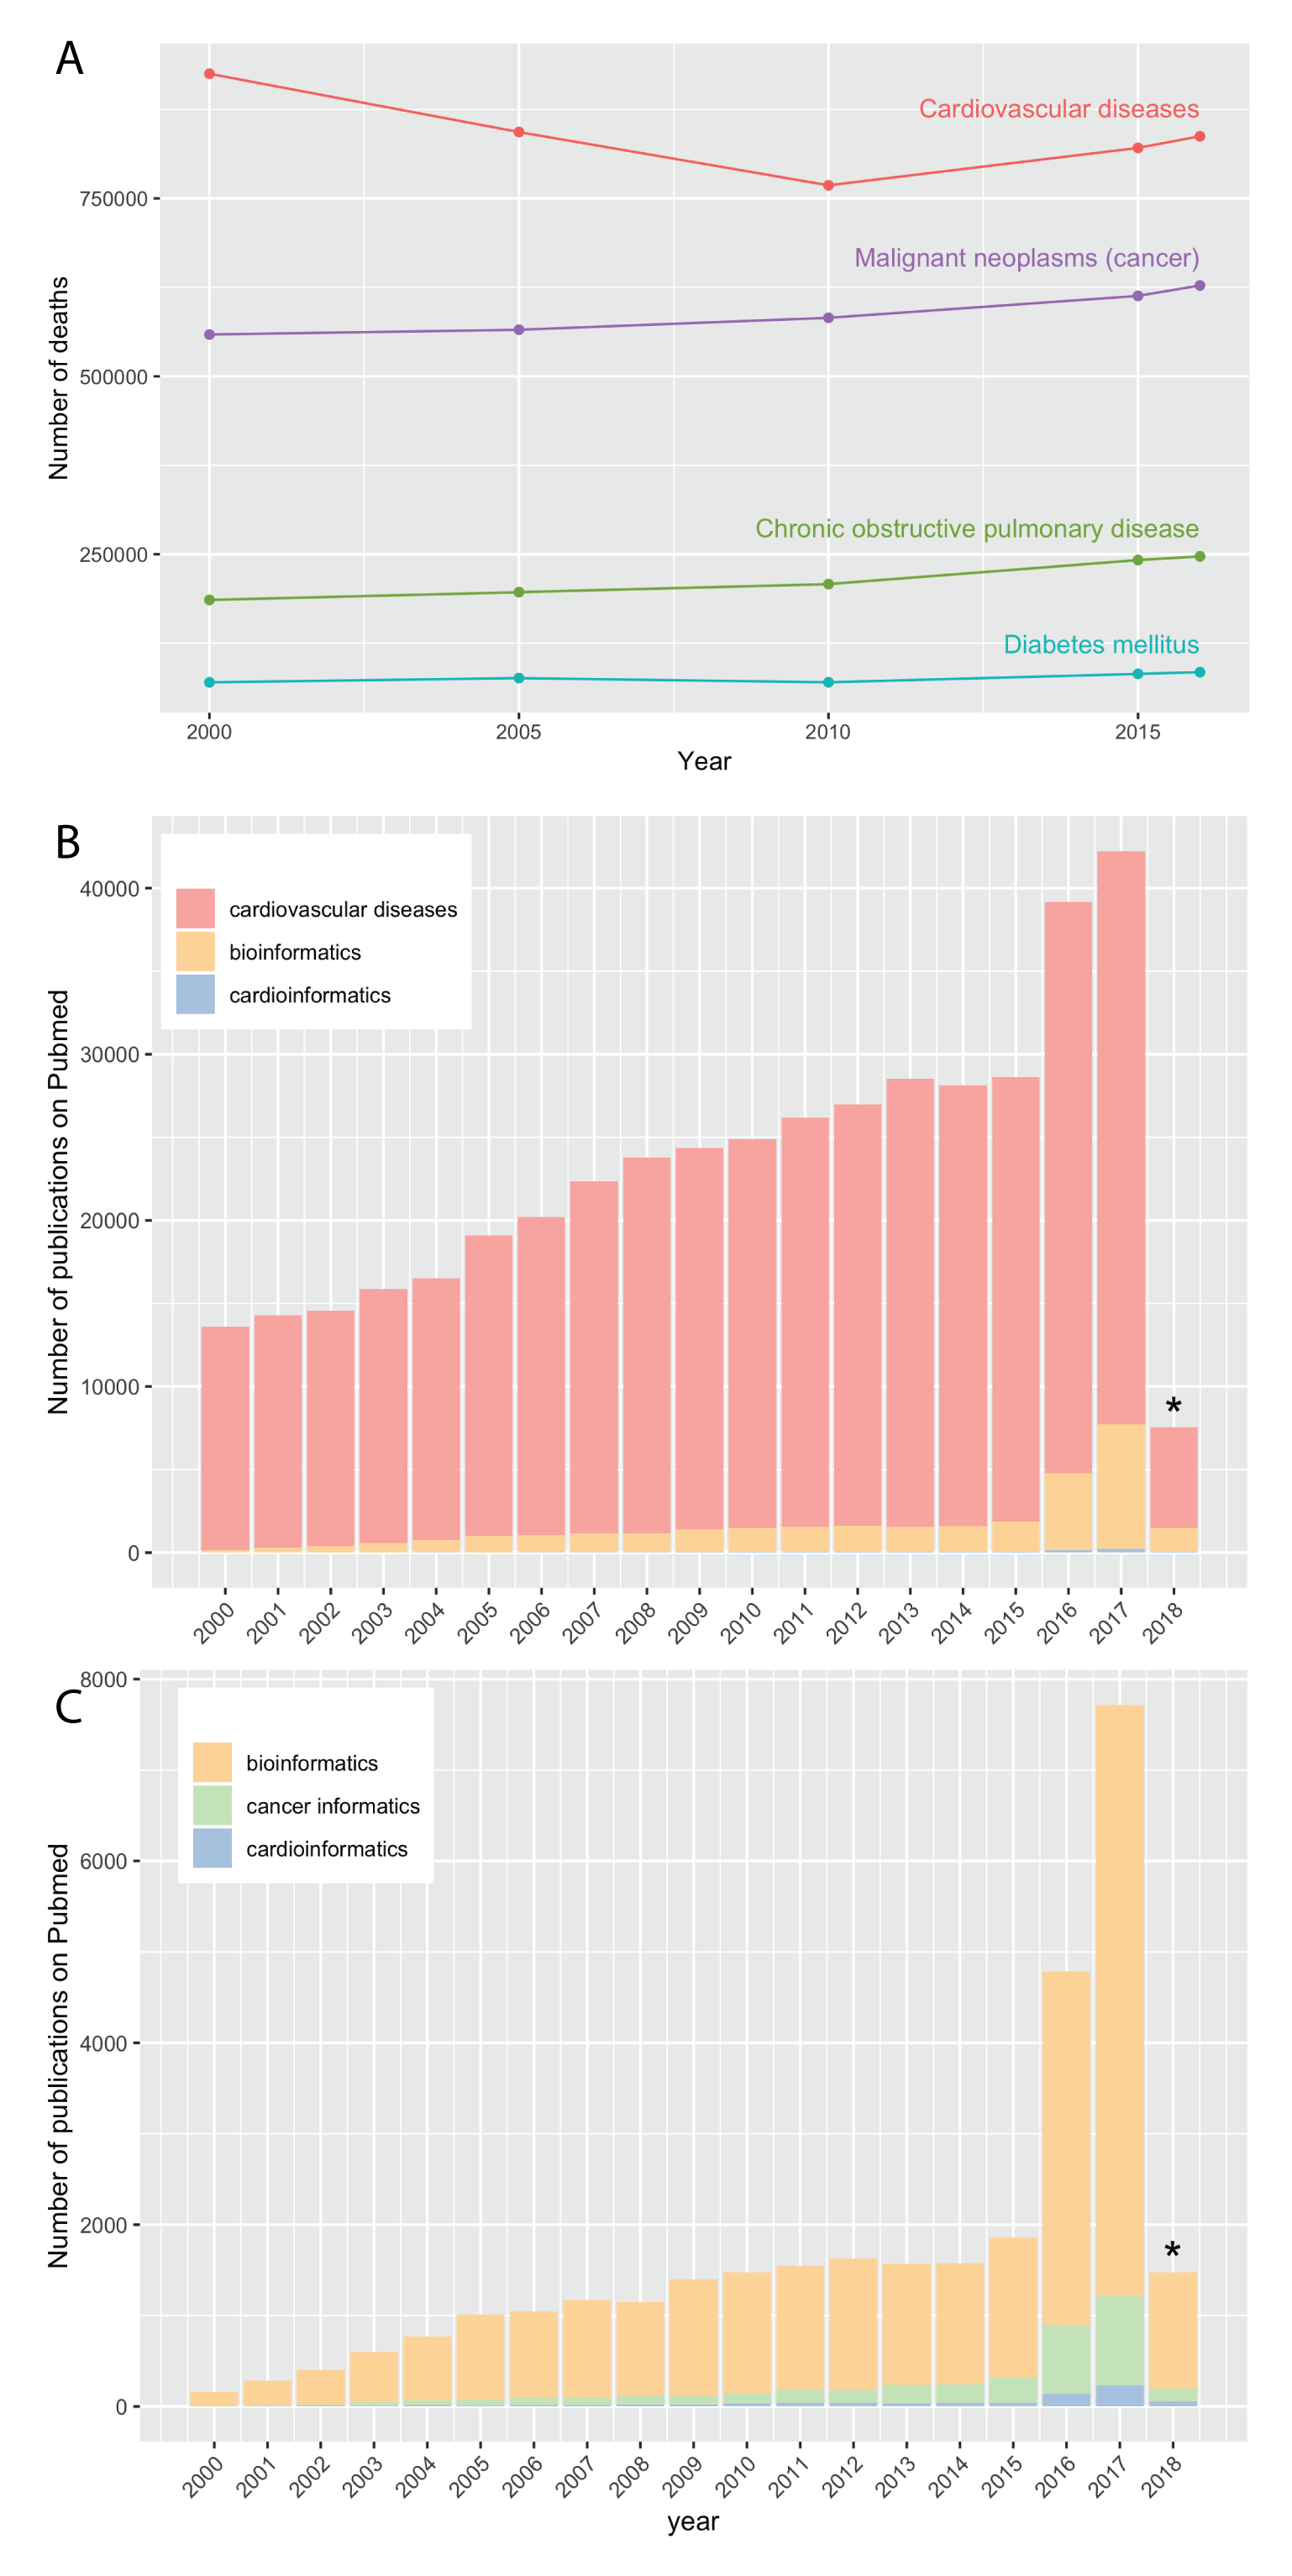
\includegraphics[width=1\linewidth]{figure1}
	\caption{\textbf{(A)} Number of deaths by Non-Communicable Diseases in the US.  Cardiovascular disease deaths have significantly surpassed cancer mortality rates since the year 2000.  \textbf{(B)} Text mining PubMed reveals that out of the total body of CVD research published in peer-reviewed journals, only a vanishingly small percentage include bioinformatics techniques or methodologies as part of the study design.  Likewise, there are far more CVD papers released annually than bioinformatics papers (in any domain area, not just CVD), highlighting the tremendous momentum and volume of new research results published in the CVD field.  Nevertheless, only a small percentage of that total CVD literature includes bioinformatics techniques.  \textbf{(C) Relative to the total pool of bioinformatics papers (in any field), there are far more cancer papers that utilize bioinformatics methods than CVD papers that utilize such methods.}\\
	* Since all the queries are based on manual MeSH catalog, 2018 tallies will lag behind the true volume of publication.}
	\label{fig:figure1}
\end{figure}


Among these CVD outputs, the share of bioinformatics research has remained modest -- at least relative to comparable work done in cancer biology (Figure \ref{fig:figure1}C). While bioinformatics is at the center of precision medicine \citep{Gomez-Lopez:2017:Precision} and cardiovascular research is at the forefront of existing precision medicine initiatives, including recent Chan Zuckerberg Biohub funding for CVD projects such as ``Multi-scale deep learning and single-cell models of cardiovascular health", the field of cardioinformatics is still in its early days with ample opportunities to benefit from cutting-edge data science techniques and machine learning (ML) methodologies, as has been the case in oncology.  Even now, the application of ML is already being recognized as indispensable in many aspects of cardiology \citep{Shameer:2017:Translational,Shameer:2018:Machine} and, therefore, given the availability of increasingly performant ML implementations \citep{MLPerf:2018:MLPerf}, cardioinformatics is better positioned to tackle domain-specific research questions by developing clinical applications to enhance compute-intensive tasks such as those found in medical imaging, CVD risk prediction modeling, among other active research areas. In general, efficient implementations of advanced computational algorithms that optimize for time, cost, and accuracy measures across broad domains of biological data science, such as single-cell sequencing \hl{(cite Becht et al. 2018)} or long-read mapping \hl{(cite Heng Li's Minimap2 Bioinformatics paper)}, will find increasingly more adoption in CVD research throughout the next few years as journals such as \emph{Genome Biology} begin gearing up for the release of special issues dedicated exclusively to performance benchmarking of new and existing software tools.  Taken together, programmatic need for bioinformatics benchmarking and awareness of state-of-the-art tools for performing CVD research will bridge across multiple areas of expertise (e.g., single-cell sequencing technologies, long-read mapping, 3D genome visualization, etc.), making cardioinformatics research a truly multi-disciplinary initiative for dissecting the molecular mechanisms behind complex CVD traits.   


Recently, the American Heart Association (AHA) Institute for Precision Cardiovascular Medicine partnered with Amazon Web Services to provide a variety of grant funding opportunities for testing and refining artificial intelligence and machine learning algorithms using healthcare system data and multiple longitudinal data sources to fund research that improves our understanding of all CVD data related to precision medicine.  Therefore, we expect that grant funding initiatives such as these will gradually begin narrowing the gap between cardioinformatics and cancer research in terms of the availability of improved computational tools, infrastructure, and analysis resources.  Some recent trends in this direction include large-scale infrastructure and knowledge portal development \citep{Kass-Hout:2018:American, Khomtchouk:2018:HeartBioPortal, Broad:NA:Cardiovascular, Broad:NA:Cerebrovascular} for working with CVD data, as well as population-wide multi-omics initiatives such as the NHLBI Trans-Omics for Precision Medicine (TOPMed) Consortium \citep{NHLBI:2014:TransOmics} for integrating whole-genome sequencing (WGS) and other -omics data (e.g., metabolic profiles, protein and RNA expression patterns) with molecular, behavioral, imaging, environmental, and clinical data.  In this review, we highlight these contemporary opportunities and perspectives for CVD genomic and precision medicine research, introduce the bountiful resources available and propose ways to advance this field further by promoting a culture steeped in computation vis-\`{a}-vis modern bioinformatics methodologies.


\section*{The democratization of data and the rise of knowledge bases}

The last few years have seen a meteoric rise in the availability of computational resources and infrastructure that provide access to aggregate genetic data and genomic summary results to facilitate rapid and open sharing of individual level data and summary statistics pertinent to various biological diseases and data types.  One of the early pioneers of web-based knowledge portals has been a Memorial Sloan Kettering Cancer Center resource called cBioPortal \citep{Cerami:2012:cBio,Gao:2013:Integrative}, which provides intuitive visualization and analysis of large-scale cancer genomics datasets from large consortium efforts such as TCGA \citep{TheCancerGenomeAtlasResearchNetwork:2013:Cancer} and TARGET \citep{Koscielny:2017:Open} as well as publications from individual labs.  Other major players in the cancer knowledge base arena include the National Cancer Institute's Genomic Data Commons (GDC) Portal \citep{Grossman:2016:Shared,Jensen:2017:NCI}, which provides full-download and access to all raw data (e.g., mRNA expression files, full segmented copy number variant files, etc.) generated by TCGA and TARGET.
%% SCP does not focus on cancer
%In addition, resources such as the Broad Institute's Single Cell Portal \citep{Broad:NA:Single} provide an unprecedented view into the biology of cancers like glioblastoma at a single-cell sequencing level.    
	
More recently, the Knowledge Portal Network Group at the Broad Institute has started implementing a wide variety of complex disease knowledge bases focused on type II diabetes, sleep disorders, cardiovascular and cerebrovascular diseases.  The purpose of these resources is to aggregate and store statistical data for billions of genetic variants and organize them to be rapidly queried and visualized by biologists, statistical geneticists, pharmaceutical researchers, and clinicians to find genetic associations, treatment targets, etc.  Other such knowledge bases focused on exploring large-scale genetic association data in the context of, for instance, drug/treatment targets include the OpenTargets initiative \citep{Koscielny:2017:Open}, which is a public-private venture that generates evidence on the validity of therapeutic targets based on genome-scale experiments and analysis.  Similarly, the Accelerating Medicines Partnership-Alzheimer's Disease (AMP-AD) Target Discovery and Preclinical Validation Project has developed an AMP-AD Knowledge Portal to help researchers identify potential drug targets to accelerate pre-competitive Alzheimer's disease treatment and prevention \citep{NIA:2015:AMP}.  
	
	In addition to these various genetic association efforts, CVD knowledge bases such as HeartBioPortal \citep{Khomtchouk:2018:HeartBioPortal} have begun integrating gene expression information with genetic association information, motivated by the stimulus that transcriptomic data provide powerful insights into the effects of genetic variation on gene expression and alternative splicing in both health and disease.  Such large-scale integrative multi-omics efforts to dissect the molecular mechanisms behind complex disease traits now also extend beyond academia into biotech startup companies, non-profits, and initiatives such as Research to the People, Quiltomics, Omicsoft, Omics Data Automation, Occamzrazor, NextBio, BenevolentAI, Insitro, Researchably, and others -- many of which have successfully been acquired by larger biotech companies such as Illumina, Qiagen, etc.  Therefore, the biological data science world has started moving progressively closer towards large-scale integration of knowledge bases, rather than just individual studies or datasets.  Parallel to these academic and industry initiatives, several government-led genomic sequencing programs to collect a country's patient data have appeared over the years to build a centralized database for disease prevention, health management and discovery, e.g., the recently completed \textit{100K Genomes Project} in the UK \citep{Caulfield:2017:100K} or the ongoing \textit{100K Wellness Pioneer Project} in China \hl{(Trang, cite this)}, NIH's \textit{All of Us Research Program} \citep{NIH:2018:All} and the Department of Veterans Affairs Million Veterans Program \citep{Gaziano:2016:Million} in the US, many of which contain vast quantities of population-wide race/ethnic group-specific cardiovascular disease data.  


		\begin{figure*}[!tpb]
		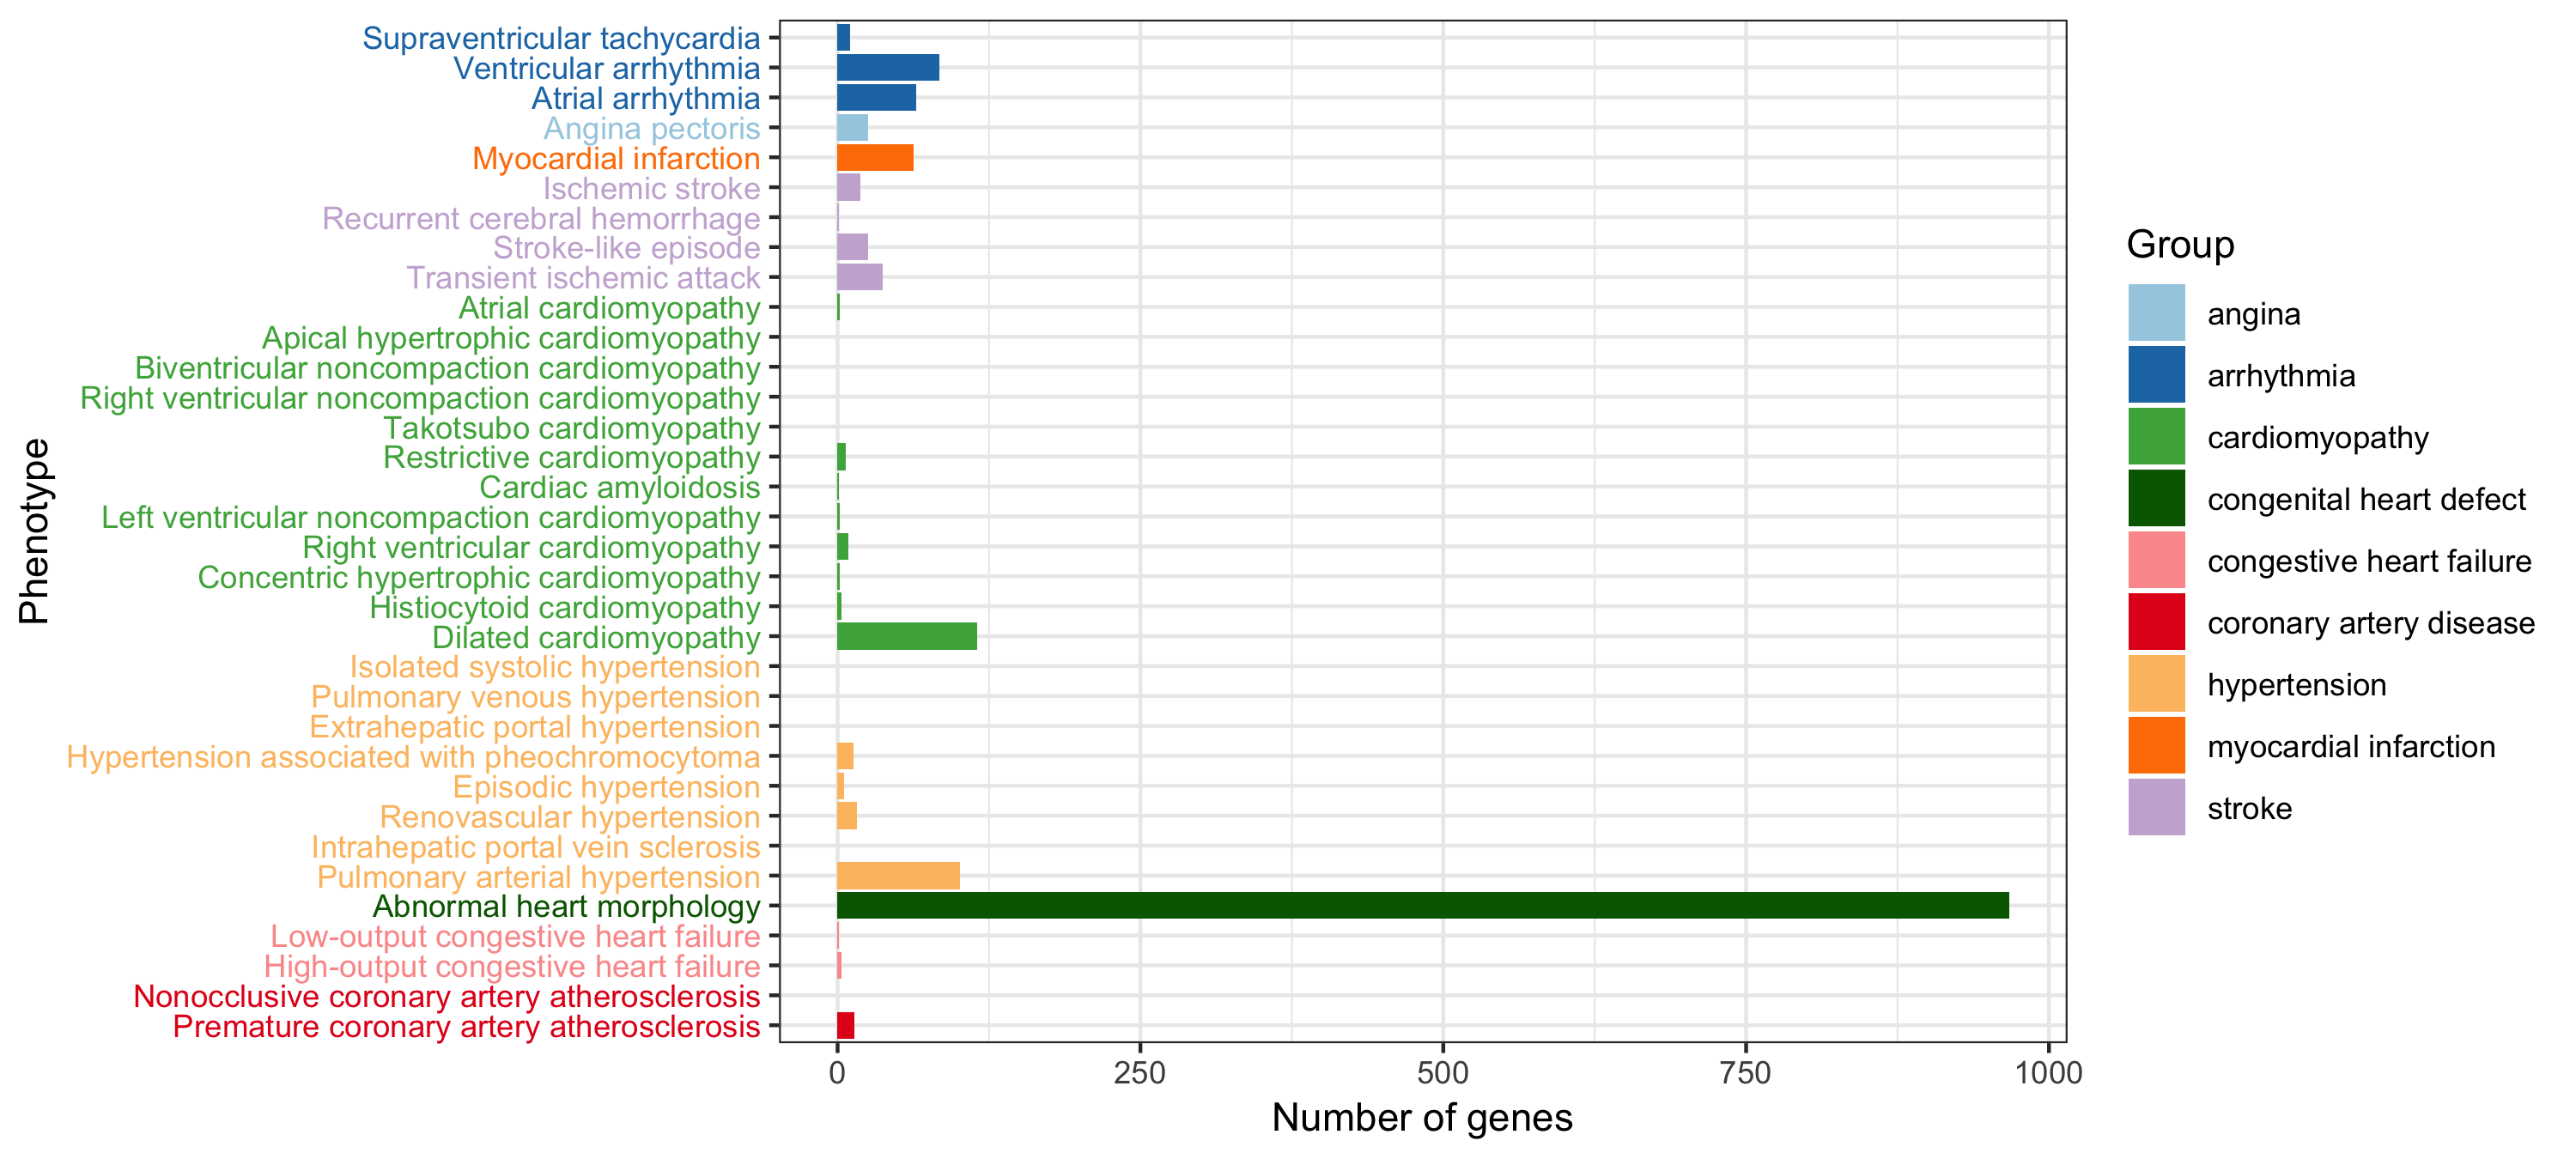
\includegraphics[width=1.\linewidth]{hpo-gene-count}
		\caption{The number of genes associated with \emph{``Abnormality of the cardiovascular system"} (HP:0001626) as reported in the Human Phenotype Ontology \citep{Kohler:2014:Human},
			 with phenotype annotations pooled from OMIM \citep{McKusick:2018:OMIM} , Orphanet \citep{INSERM:1997:Orphanet}  and DECIPHER \citep{Firth:2009:DECIPHER}.}
		\label{fig:hpo_gene_count}	
	\end{figure*}
	
	
	
	
	\section*{Complexity of CVDs}  % the problems
	\subsection*{The number of actors}
	
	% large number --> small effects
	% large number --> more interactions, intra and inter-pathways
	% 
There is a certain genetic component in all major categories of heart disease (Figure \ref{fig:hpo_gene_count}).  As more studies are published, the number of genes found associated with a disease has also increased and, in most cases, gone beyond a few genes that could be described in a single-page table or diagram.  Dilated cardiomyopathy (DCM), the most common cause of heart transplantation, is a vivid example of how causal variants and their corresponding genes were discovered over the years.  In a recent review \citep{Burke:2016:Clinical}, 16 disease-causing genes were compiled, along with an additional 41 putative genes.  Meanwhile, the NHGRI-EBI GWAS Catalog \citep{MacArthur:2017:new} and annotations on Human Phenotype Ontology \citep{Kohler:2017:Human} suggested a much larger number of genes associated with this condition, 69 genes and 115 genes, respectively.  Clinical application has been keeping up, with a typical commercial gene panel for DCM genetic testing covering 50 genes on average, and 111 in total \citep{McNally:2017:Dilated}.  Since it is reasonably expected that when more genes are involved in a disease, the individual effect exerted by each gene gets smaller, these constantly expanding gene panels suggest that the risks conferred by mutations in a single gene are less likely to be indicative of the disease risk.  For example, the Stockholm-Tartu Atherosclerosis Reverse Networks Engineering Task study (STARNET) \citep{Franzen:2016:Cardiometabolic} asserted the negative correlation between minor allele frequency and the effect size across all tissues (liver, skeletal muscle, adipose tissue, atherosclerotic aortic root, artery and blood).  From a research perspective, these findings imply that the quest of pinpointing causal variants is getting more challenging, because testing the variant-phenotype association on small-effect variations requires a much larger number of samples for sufficient power, or critically different methods of statistical testing and inference. Genetic varaints\hl{(Tim, would you like to include a word or two on Mendelian randomization and instrumental variable analysis here?)}
	
	
Besides the increasing difficulty of discovering these genes, modeling their effects poses its own unique set of challenges. With a potential interaction between every pair of genomic features, be they genes or regulatory sequences, the number of such interactions increase quadratically with the number of actors, leading to the combinatorial explosion of states that a biological system can assume.  Moreover, ethnicity and ancestry-specific differences add a further layer of complexity. \hl{(Tim, would you care to elaborate more here?)}
	
The number of genes or regulatory elements contributing to CVD risks will likely inflate beyond those directly associated with diseased traits, due to the highly interconnected wiring of biological pathways.  For instance, independent research in aging has unraveled the intertwined relationship between heart disease and longevity pathways \citep{North:2012:Intersection}.  With age being the most important factor in constituting cardiovascular disease risk \citep{Steenman:2017:Cardiac}, it is unavoidable that these longevity genes will be involved in future analyses of CVD genetics. The genetic scope of these diseases may be enlarged even further to include most of the genome, under the recently proposed omnigenic model for complex traits, in which most heritability is explained by peripheral genes outside of the core pathways \citep{Boyle:2017:Expanded}. Such expansion calls for a paradigm shift from additive effects of multiple genes to the interactions between them, from the physical genes to the "eigen-genes" that represent biologically functional modules \citep{Weiss:2012:Good}.
% From a historical perspective, when thousands of loci were found to be involved in a single disease, the paradigm shifted from additive effects of multiple-genes to the interactions between them, turning the focus from physical genes to the "eigengenes" that represent biologically functional modules \citep{Weiss:2012:Good}. The ability to view and compute on biological systems as a whole allows one to focus on the effects of a drug without the mechanistic knowledge of individual actors and their interactions. From a research perspective, such approaches are also helpful for understanding a system by ways of its response to external stimuli. 
	
As with other complex diseases, missing heritability has been a long-standing puzzle in cardiovascular disease \citep{Manolio:2009:Finding}. Despite the early successes in pinpointing the causes of several monogenic diseases, the large body of genome-wide association studies have defied many widely-held beliefs about genetic variants in humans, hinting at various directions to search for the missing heritability.  The most trivial situation where inherited risk is not fully accounted for is when the variants are simply too rare to be detected with sufficient power. One addresses this issue by collecting more samples or improving statistical tests \citep{Zuk:2014:Searching}.  This reason has driven a lot of efforts to enlarge and diversify the study population, where the availability of a large number of genomes and exomes are currently enabling the search for rare variants, as embodied by ongoing large-scale consortium efforts such as the Million Veterans Project \citep{Gaziano:2016:Million}, ExAC then gnomAD \citep{Lek:2016:Analysis}. The other directions to search for missing heritability require one to move beyond the exome and genome, as discussed in the next section.
	
	
	%does it help to have too many variants in a genetic risk score?
	
	
\subsection*{The diversity of actors in an era of trans-omics}

\subsubsection*{From SNPs to structural variations}
	
	%\begin{figure*}[!tpb]
		%	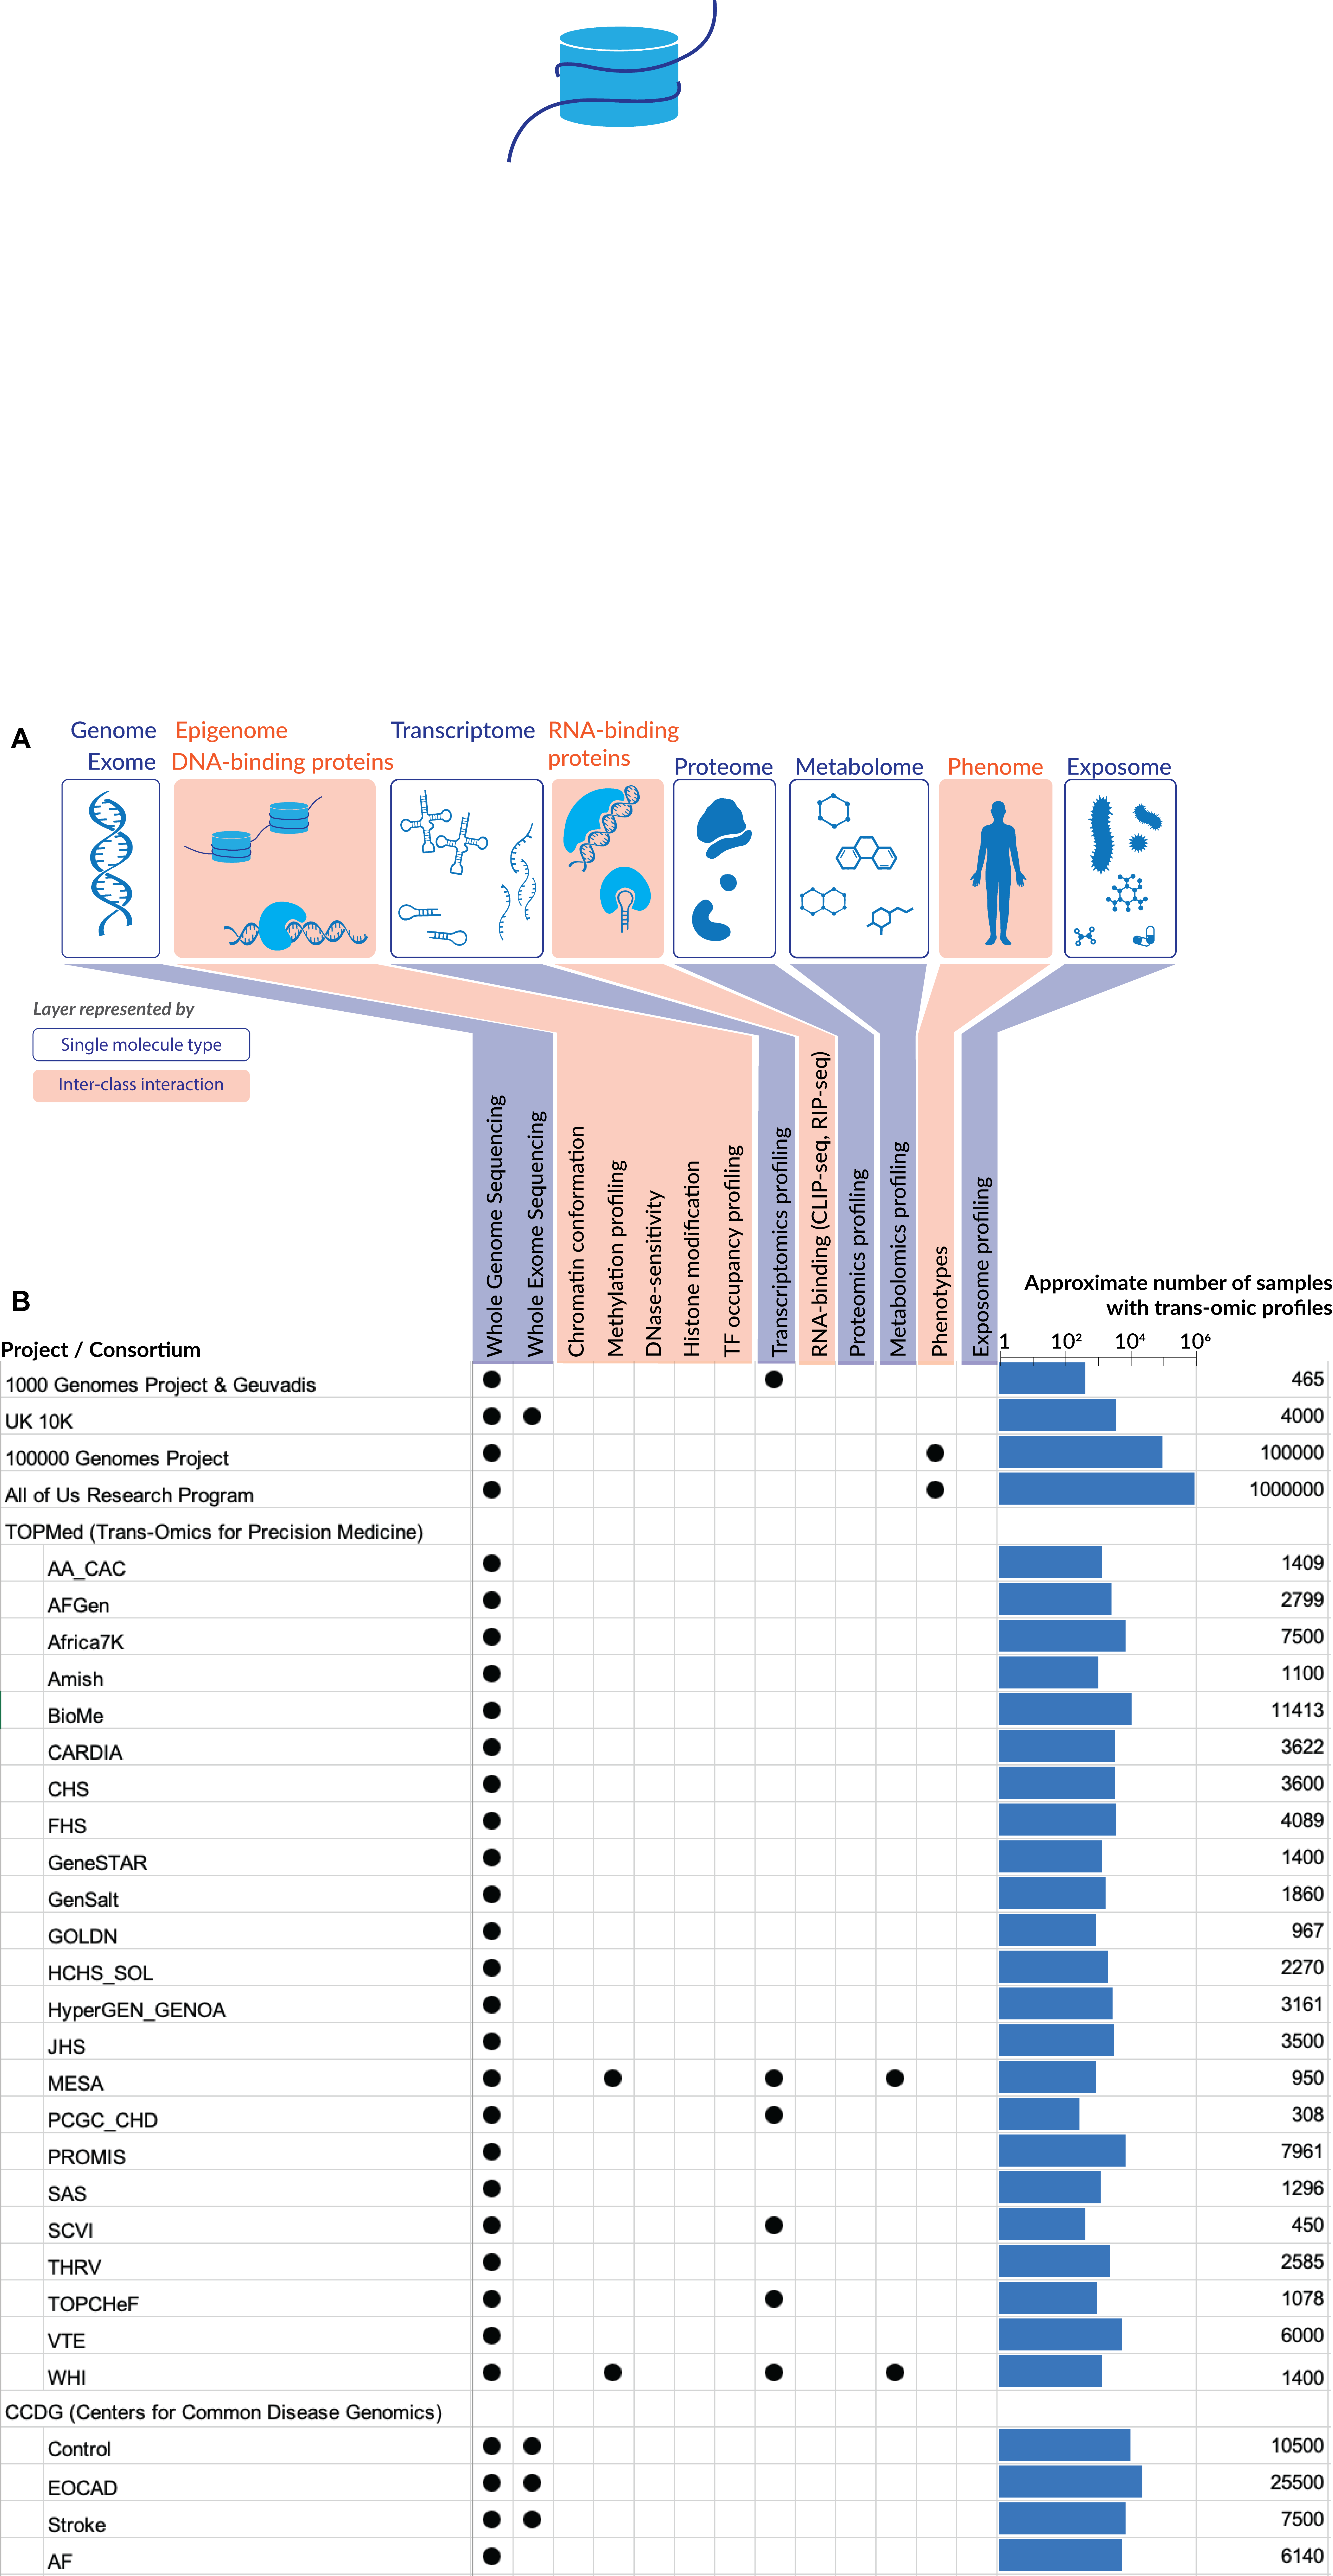
\includegraphics[width=1\linewidth]{multiomics}
		%\rule{2cm}{2cm}
		%\caption{PLACE HOLDER - layers of omics data and the corresponding molecular assays. \comment{Genome, epigenome, transcriptome, proteome, metabolome, microbiome, exposome}}
		%\label{fig:multiomics}
	%\end{figure*} 
	
	% Our understanding of CVD has been critically limited by the technical capability in characterizing various molecular fractions of a cell \hl{(this sounds like the perfect moment to discuss the impact that single-cell sequencing has had in CVD)}.
	Historically, genome-wide association studies were predominantly conducted on single-nucleotide polymorphisms (SNPs) thanks to the availability of easy-to-produce SNP microarrays. Such technologies have clearly enriched our knowledge base of single nucleotide variants, while leaving structural variations poorly understood. There are now 660 million SNPs documented in the dbSNP database \citep{NCBI:2018:dbSNP}, compared to 4.6 million structural variations in the DGVa (Database of Genomic Variants archive \citep{EMBL-EBI:2018:Database}, which also includes studies annotated by the NCBI-hosted database of structural variants, dbVar \citep{NCBI:2018:dbVar}).  Structural variation (SV) databases such as dbVar and DGVa are in fact storing each study-publication individually instead of cataloging structural variations into data entries. Although the current knowledge base of structural variations is not sufficient to create reference entries of SV, the map of SV from 1000 Genomes Project \citep{Sudmant:2015:integrated} has enabled further studies of the role of SV in cardiac diseases, suggesting the potential impact of SV on the transcriptional regulation of cardiac genes expressed in the heart \citep{Haas:2018:Genomic}. As envisioned, structural variations might be one of the promising areas to look for the missing heritability in CVD \citep{Eichler:2010:Missing}.  To this end, projects like TOPMed contain a Structural Variant Working Group to call copy-number variants (CNVs) within TOPMed, and they have begun incorporating large-scale multi-ancestry studies spanning diverse types of sequencing data from both European and non-European race/ethnic groups.  For instance, the Multi-Ethnic Study of Atherosclerosis (MESA) study \citep{Bild:2002:MultiEthnic} within TOPMed includes WGS, RNA-seq, metabolomics, proteomics, and methylomics data across a variety of multi-ethnic communities (white, Hispanic, African-American, and Asian).  Specifically, MESA investigates the characteristics of subclinical cardiovascular disease (disease detected non-invasively before it has produced clinical signs and symptoms) and the risk factors that predict progression to clinically overt cardiovascular disease or progression of the subclinical disease.  Likewise, the Women's Health Intiative (WHI) study \citep{NHLBI:1991:Women} within TOPMed currently includes WGS, RNA-seq, metabolomics, and methylomics data.  In general, improved risk prediction methods such as polygenic risk scores (PRS) are being used to improve our ability to predict future CVD events \citep{Goldstein:2014:Simple} based on a variety of these types of data sources, and PRS have demonstrated the ability to serve as a biomarker that is predictive of clinical outcomes to the same degree as some traditional cardiovascular risk factors (e.g., cholesterol, smoking, obesity, etc.) \citep{deVries:2015:Incremental}. 
	
	\begin{figure}[!tpb]
		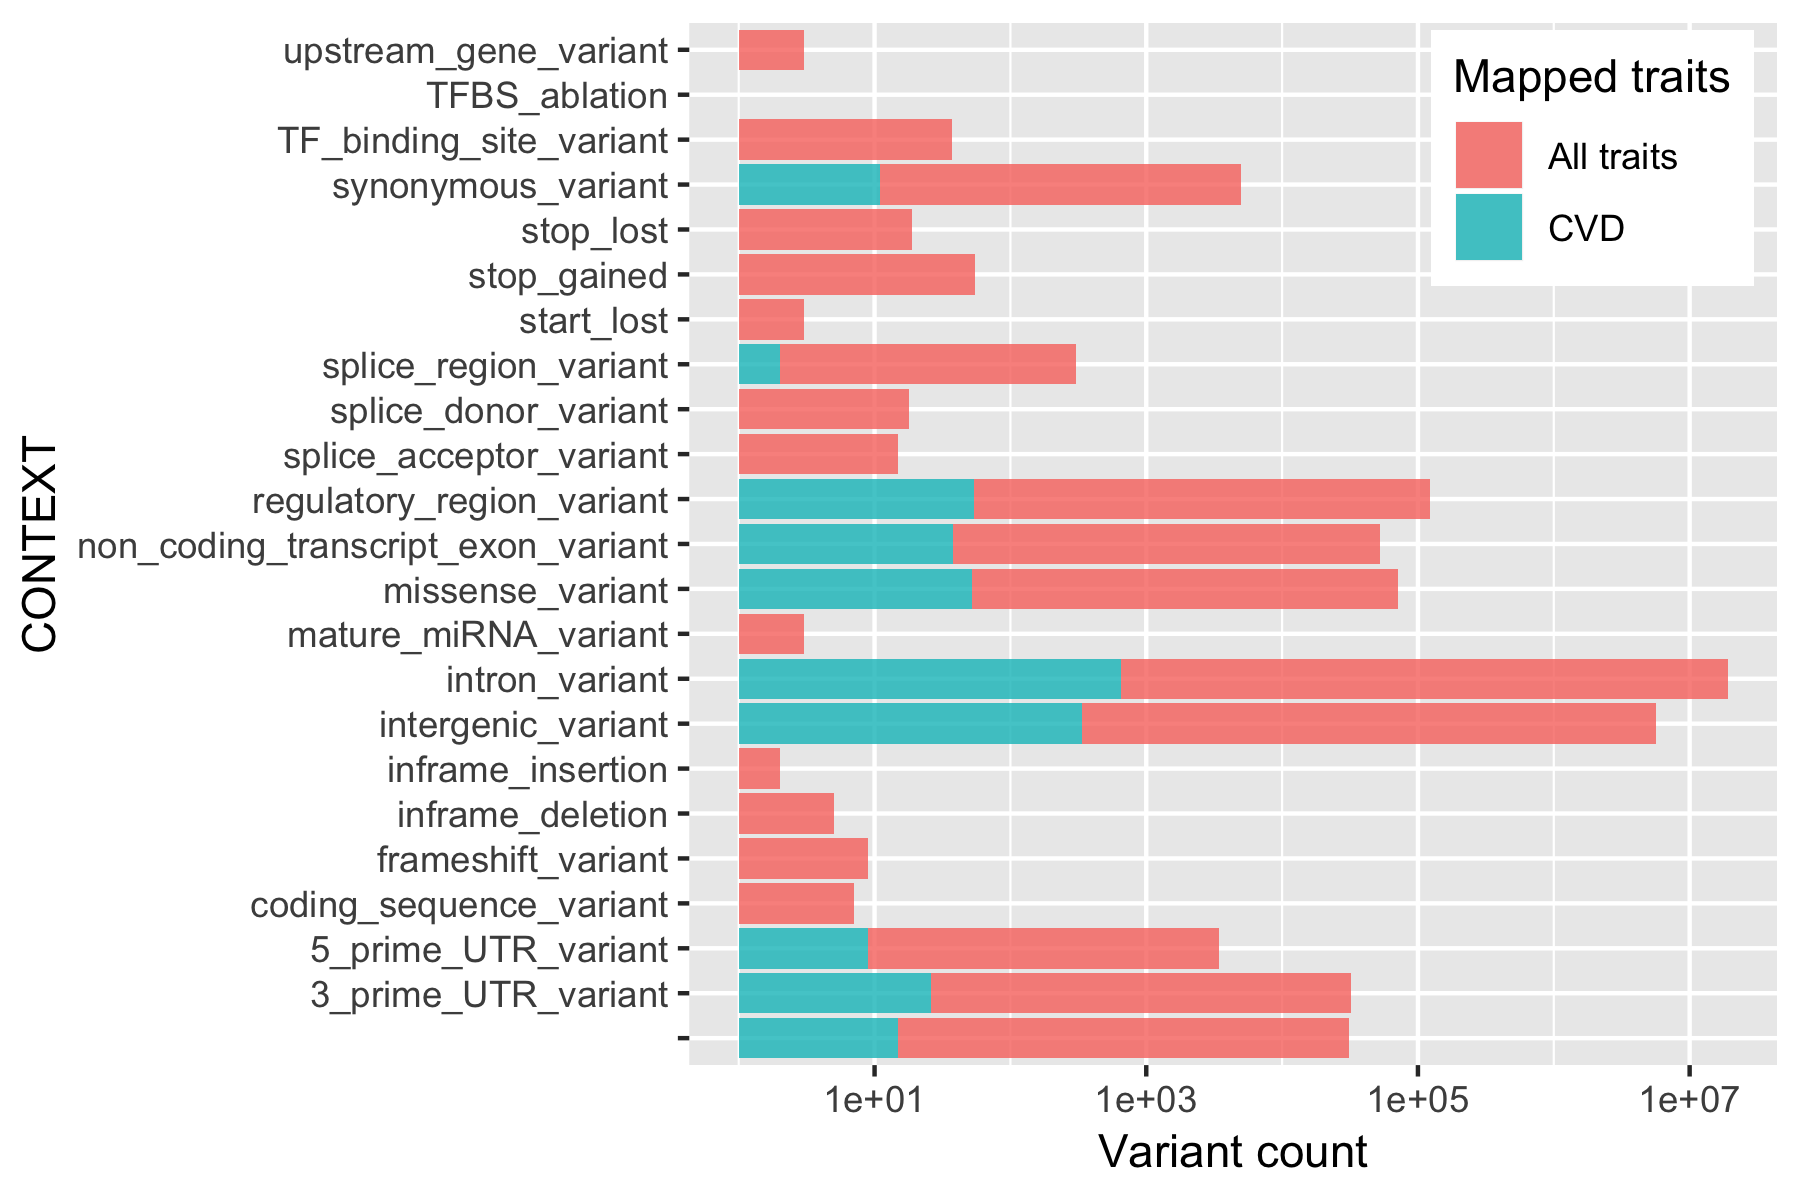
\includegraphics[width=1\linewidth]{variant_contexts}
		\caption{Distribution of SNPs that have been associated with a phenotypic trait in the human genome. The associations are downloaded from NHGRI-EBI GWAS Catalog in which only those with p-value less than $10^{-5}$ were retained.}
		\label{fig:variant_context}
	\end{figure}
	

\subsubsection*{From coding to noncoding regions}	
	As array-based genotyping was gradually replaced by next-generation sequencing, the cost of sequencing an \textit{exome}, the protein-coding part of a genome, became much more affordable and enabled the collection of more than 60000 exomes \citep{Lek:2016:Analysis}. Using this dataset, \cite{Walsh:2017:Reassessment} found that many genetic variants associated with various cardiomyopathies turned out to be equally common in clinical cases as in the control population. Genes that were consistently included on genetic testing panels for DCM such as MYBPC3, MYH6, SCN5A, etc. turned out to contribute much less etiology than previously thought, in consideration of their frequency in the control population.  The rationale for prioritizing the sequencing of exome over that of the entire genome was originally based on a regularly cited statement that the exome harbors 85\% of disease-causing variants \citep{Antonarakis:2001:nature} which turned out to be an outdated estimate from 1995. In our own survey of the NHGRI-EBI GWAS Catalog \citep{MacArthur:2017:new}, a large fraction of variants tend to occur in non-protein coding regions such as intronic, intergenic, and splice junctions (Figure \ref{fig:variant_context}). The distribution of CVD-associated variants are similar to that of all variants across the human genome. Previous studies also asserted the prevalence of regulatory regions among variants associated with cardiometabolic risk \citep{Franzen:2016:Cardiometabolic}, as well as many other complex traits \citep{Pickrell:2014:Joint}. As an unprecedented amount of whole-genome sequencing data become available from large-scale genomic projects such as \textit{The 1000 Genomes Project} \citep{1000G:2015:global}, \textit{UK10K} \citep{TheUK10KConsortium:2015:UK10K}, \textit{The 100,000 Genomes Project} \citep{Caulfield:2017:100K}, \textit{All of Us Research Program} \citep{NIH:2018:All}, TOPMed \citep{NHLBI:2014:TransOmics}, and CCDG \citep{NHGRI:2016:CCDG}, we are poised to learn more about this dark matter in the human genome and how it works in complex diseases. \hl{(Trang, include 100K Wellness Pioneer Project citation too)}

\subsubsection*{Beyond genetics: epigenetics and the gene-environment interplay}	
	Cardiovascular risks can be conferred through heritable changes in gene expression without alterations in the DNA sequence.  These epigenetic processes traditionally involve DNA methylation, a wide range of histone modifications including acetylation, methylation, phosphorylation, ubiquitylation, sumoylation and biotinylation, and are now encompassing a loosely-defined group of processes mediated by long noncoding RNAs (lncRNA). Dysregulation in epigenetic processes has been associated with the pathogenesis of cancer and many other diseases. Epigenetic mechanisms have been demonstrated to be involved in a variety of cardiovascular diseases and conditions \citep{Udali:2013:Cardiovascular,AbiKhalil:2014:emerging,Muka:2016:role,Gidlof:2016:Ischemic}.
	For instance, early differential epigenomic analysis, albeit on a limited number of samples, established differentiating features in DNA methylation and histone H3 methylation between control and failing hearts \citep{Movassagh:2011:Distinct}. Following these early findings, epigenome-wide association studies are proposing a number of DNA methylation sites associated with blood lipid \citep{Irvin:2014:Epigenomewide}, body mass index \citep{Dick:2014:DNA, Wahl:2017:Epigenomewide}, heart failure \citep{Meder:2017:EpigenomeWide}, and heart attack history \citep{Rask-Andersen:2016:Epigenomewide}. In addition, alterations in chromatin structure have been shown to induce heart failure \citep{Rosa-Garrido:2017:HighResolution}.  As more lncRNAs were discovered and characterized, the prevalence of these molecules in cardiovascular biology also emerged.
	At least 22 lncRNAs were reportedly dysregulated in CVDs including coronary artery disease, myocardial infarction, cardiac hypertrophy and atherosclerosis, affecting a wide range of molecular, cellular and physiological processes \citep{Das:2018:Deciphering, Xu:2018:Targeting}. Due to low relative abundance levels and highly tissue-specific expression patterns, lncRNAs are still challenging to study.
	While a catalog of lncRNA functions is not yet complete, some of the functions have been recognized including imprinting, scaffolding, enhancer, and molecular sponges. These actions mark the presence of lncRNAs in many cardiovascular processes such as cardiac differentiation, macrophage activation and sarcomere development \citep{Sallam:2018:Long}.
	With 107,039 lncRNAs detected in the human genome so far (reported by LNCipedia \citep{Volders:2018:LNCipedia}, as of November 2018), more lncRNAs are likely to be found involved in cardiovascular biology, hence promising potential therapeutic targets.

	%Epigenetic studies supplemented significant mechanistic insights to understand complex conditions  such as atherosclerosis \citep{Xu:2018:Targeting}. 
	
	As epigenetic processes include various molecular processes, the experimental assays for mapping of the epigenome are accordingly diverse. DNA methylation profiling can be done with methylation-sensitive restriction enzymes, bisulfite sequencing, or immunoprecipitation with antibodies against methylated-cytosine \citep{Bibikova:2010:Genomewide}. Histone modifications can be profiled by immunoprecipitation with antibodies specific to the modified histone of interest, essentially requiring a ChIP experiment for each of the histone modifications one wants to interrogate. Meanwhile, the noncoding RNA transcripts can be profiled with variations of RNA-seq experiments that are optimized for the target fraction of RNA. Such diversity entails significant difficulty in comprehensive profiling of the epigenome in a single experimental assay, stressing the need for re-collection and re-analysis of dispersed datasets for a more complete picture. As epigenetic alterations have been found responsive to environmental cue throughout life, the epigenome lays an important bridge between the genetic makeup of an organism and its phenotype by helping to explain the gene-environment interplay.
	Environmental factors have been known for decades to play a critical role in cardiovascular health, such that a CVD risk prediction using lifestyle variables performs much better than a gene-count score \citep{Joyner:2011:Ten}. Although such gene-environment interaction is of focal interest to cardiovascular epidemiology, the understanding of this relation at the molecular level has been restricted due to the difficulties in measuring the exposome, i.e. all environmental exposures throughout life, including an individual's diet, pollutants, and infections \citep{Wild:2005:Complementing}. With recent development of wearable device to collect real-time data in a non-intrusive manner, it is now possible to monitor the exposome for its dynamic compositions of chemical compounds and micro-organisms \citep{Warth:2017:ExposomeScale, Jiang:2018:Dynamic}. Being among complex traits that are heavily influenced by environmental factors, cardiovascular diseases are especially well-positioned to benefit from these advances.
	
	\section*{The challenges of cardioinformatics}
	As illustrated in the previous section, the complexity of cardiovascular diseases calls for pushing research beyond traditional territories.
	Such expansion implies the inclusion of various data modalities, such as genome sequence, DNA-methylation profiles, RNA expression profiles, protein expression profiles, metabolic profiles, etc. (Figure \ref{fig:trans-omics} to analysis workflows. These modalities represent different classes of biological molecules as well as their interactions (Figure \ref{fig:trans-omics}A). While benefiting from two decades of research in bioinformatics, cardioinformatics is presented with a unique set of challenges shaped by the current landscape of contemporary research. From our own perspective, we suggest three particularly pertinent areas to prioritize cardioinformatics research: data sharing/security, multi-omics analysis, and augmented intelligence.
	
	%From our own perspective, we suggest three key challenges that are particularly pertinent to cardioinformatics, corresponding to three stages of research: obtaining the data, analyzing them and conveying the knowledge.
	
	
	\subsection*{To share or not to share}
	
	Data sharing is believed to help scientific advances, thus benefiting everyone. The sharing of personal health and medical data, however, comes with the risk of compromising a person's privacy and subjecting them to discrimination.  The current data governance practice employs several administrative measures in the hope of minimizing the risk of exposing the data to adversity, or bad intentions. Taking the process of dbGaP data requests as an example: to access 658,305 records of genotype-phenotype data (Table \ref{tab:dbgapSubject}) potentially relevant to future biomedical studies, a researcher first needs to browse these datasets, determine whether each dataset is consented for its purpose, obtain IRB approval if necessary, then file a request, prepare the facility, implement the security measures, and transfer the data upon approval. Although the data users are advised, for example, to "avoid placing data on mobile devices" and "destroy [the data] if they are no longer used or needed", the only guarantee to such compliance is the vigilant mindset of every researcher involved in the data behind the project.  In addition, datasets are associated with different types of consents, dictating what purposes are permitted, for example general research, disease-specific research, or biomedical research. Therefore, data users are responsible for obtaining the IRB approval compatible with these consents. These regulatory requirements have heightened the barrier to data access albeit without robust mechanisms to enforce data protection nor to revoke the access when necessary.  To add to these challenges, before filing a request, one needs to dive into the metadata of individual studies and decide which datasets are useful for the target research. Important information about a dataset such as the list of phenotypic variables are often vastly different from study to study and cannot be filtered against. In addition to those parameters of a study design, researchers need to be aware of the various types of consent forms applied to different datasets, many times within a single study. This procedure to obtain data access is currently applied for all controlled-access data in dbGaP, adding a significant administrative burden to biomedical researchers.

	As a pioneering effort towards more accessible biomedical data, the AHA's Precision Medicine Platform \citep{Kass-Hout:2018:American} has greatly simplified this process by streamlining the search, request and transfer of data. Datasets deposited on this platform were harmonized such that users can query for data across multiple studies by some common parameters, selectively request access to the relevant data, and perform analyses on the cloud-based workspace. The platform has lifted significant burden off data users by having them filing one request for multiple datasets, and the data owners, being aware and responsible for complying with the consents on their data, will decide whether access can be granted. The cloud-based workspace also allows data to be transferred and analyzed in a controlled environment which can be ensured to comply with regulatory standards. The risk of intellectual property being compromised remains, for the data, once transferred, cannot be withdrawn nor prevented from being copied. As recognized by the authors, the platform is "only as good as the researchers make it". \citep{Kass-Hout:2018:American}.
	More secured modes of data sharing have been explored, forming a spectrum of varying balance between analytic power and data protection. ViPAR \citep{Carter:2016:ViPAR} supports on-memory analysis of poooled data which are transferred to a central system, avoiding the permanent storage of sensitive data outside of the original sites. To eliminate all the risk and responsibilities associated with direct access of sensitive data, DataSHELD  \citep{Gaye:2014:DataSHIELD, Wilson:2017:DataSHIELD} and COINSTAC \citep{Plis:2016:COINSTAC} aimed to allow these data to be analyzed without moving out of the data owners' facility. Current implementations have shown that a variety of analytic tasks such as summary statistics, histogram, generalized linear model (DataSHIELD), gradient descent (COINSTAC) can be performed in a distributed manner to achieve equally accurate result compared to the physically pooled counterpart and more importantly, without disclosure of sensitive or personally identifiable information.
	
	Beside controlled-access data, a large amount of human data such as RNA-seq, ChIP-seq, Hi-C, etc. public domain results are freely accessible with no restrictions. Without genomic sequences, genotype or phenotype data, the processed output of these assays are deemed anonymous and void of sensitive information. However, recent studies have shown that information leakage is still possible, subjecting individuals to linking attacks that may reveal their identity \citep{Harmanci:2016:Quantification, Harmanci:2018:Analysis}.  With millions of human genomes and thousands of other omics profiles on the not-so-distant horizon, it is critical that cardioinformatic researchers pioneer the applications of these security measures, to ensure scientific advances do not compromise human rights to privacy and non-discrimination.
	
	\subsection*{Multi-omics data ocean}
    The explosion of biological data is manifested in the growth of databases, consortium efforts, repositories, as well as the amount of data hosted in those warehouses. High-throughput technologies are now available for characterizing and quantifying all major classes of biological molecules including DNA, RNA and protein, leading to the creation of centralized repositories such as Gene Expression Omnibus (GEO) \citep{Barrett:2013:NCBI} for gene expression data, dbGaP \citep{Tryka:2014:dbGaP} for genotypes and phenotypes, ProteomeXchange \citep{Vizcaino:2014:ProteomeXchange,Deutsch:2017:ProteomeXchange} for proteomics, MetabolomeXchange for metabolomics, among others.  GEO, the most popular repository for functional genomics data, has accumulated more than 100,000 studies \citep{Zhu:2008:GEOmetadb}. Among those, CVD publications have contributed more than 2000 microarray-based experiments, and about 900 high-throughput sequencing experiments for various purposes (Figure \ref{fig:geo-assay}). The amount of data potentially re-usable for CVD resdearch may be even larger, when taking into account studies that did not focus on cardiovascular disease but generated a decent number of assays on relevant biospecimens such as heart, blood or blood vessel. Among such studies are ENCODE \citep{ENCODE:2012:integrated} and Roadmap Epigenomics \citep{Roadmap:2015:Integrative}.
	Meanwhile, in dbGaP, where human genotype-phenotype data are deposited, CVD research has contributed data on 658,305 subjects, 16,786 (2.5\%) of whom had consented for the data to be employed for general research (Table \ref{tab:dbgapSubject}) (See Supplementary information for a comprehensive list of CVD studies deposited in dbGaP.)
	In addition to the central repositories for established and popular experimental methods, smaller databases with narrower focus are also budding. For instance, chromatin structure data from 3C, 4C, 5C and Hi-C experiments have been collected in dedicated databases such as 3CDB \citep{Yun:2016:3CDB} and 4DGenome \citep{Teng:2015:4DGenome}. Noncoding RNAs are being added into databases such as lncRNAdb \citep{Quek:2015:lncRNAdb}, NONCODE \citep{Fang:2018:NONCODEV5}, and LNCipedia \citep{Volders:2018:LNCipedia}.
	
	
			\begin{table}[]
	\processtable{The subject count aggregated from studies deposited in dbGaP, consented for General Research Use (GRU)
		\label{tab:dbgapSubject}}
{\begin{tabular}{l l l}
			\toprule
			& \textbf{CVD} &  \textbf{All}                         \\ \midrule
			16s rRNA (NGS)                 &     0 &      92 \\
			CNV Genotypes                  &     0 &   48972 \\
			Chromatin (NGS)                &     0 &     139 \\
			Genomic Sequence Amplicon (NGS)&     0 &       8 \\
			Methylation (CpG)              &     0 &     657 \\
			Methylome sequencing           &     0 &     152 \\
			QTL Results                    &     0 &     281 \\
			RNA Seq (NGS)                  &   333 &    1498 \\
			SNP Genotypes (Array)          &  6658 &  113597 \\
			SNP Genotypes (NGS)            &  4277 &   11786 \\
			SNP Genotypes (PCR)            &     0 &      10 \\
			SNP Genotypes (imputed)        &     0 &   29693 \\
			SNP/CNV Genotypes (NGS)        &     0 &     936 \\
			SNP/CNV Genotypes (imputed)    &     0 &    9291 \\
			SNV (.MAF)                     &     0 &       2 \\
			SNV Aggregate (.MAF)           &     0 &     570 \\
			Targeted Genome (NGS)          &     0 &    9918 \\
			Whole Exome (NGS)              &  5518 &   12771 \\
			Whole Genome (NGS)             &     0 &    1245 \\
			mRNA Expression (Array)        &     0 &     798 \\
			miRNA (NGS)                        & 0 &   228 \\ \hline
			Total subject count in data consented for GRU & 16786 & 242644 \\ \hline
			All consent groups & 658305 & Unknown \\	
		\end{tabular}}{NGS: Next-generation sequencing\\ QTL: Quantitative Trait Loci}
	\end{table}
	
	Such abundance and diversity of data promises valuable insights once the data is aggregated across studies within a given omics domain (e.g., RNA-seq), or across multiple omics domains (e.g., RNA-seq, ChIP-seq, ATAC-seq, etc.). Efforts to aggregate genomic data (both individual and summary-level statistics) have resulted in valuable datasets such as The Cancer Genome Atlas \citep{TCGA:2013:Cancer} for genomics and functional genomics data in cancer, or ExAC and gnomAD for exome and genome sequencing data \citep{Lek:2016:Analysis}. Aggregated exomes/genomes such as ExAC/gnomAD have been a valuable resource for estimating the allele frequencies of the general population as well as within various ethnic groups. With the upcoming wave of trans-omics data spanning diverse sources and sequencing types (Figure \ref{fig:trans-omics}), algorithms-based data harmonization will become a more pressing problem for cardioinformatics. Some early solutions have started to be proposed, e.g., Biochat for GEO metadata \citep{Khomtchouk:2018:Biochat}, OmicsDI for diverse datasets spanning genomics, transcriptomics, proteomics and metabolomics \citep{Perez-Riverol:2017:Discovering}.
	
	% and metadata-driven frameworks for harmonizing and analyzing AHA Precision Medicine Platform clinical trials data using an OMOP common data model \hl{(Trang, cite OMOP as well as this URL from Rocky 2018 and take the backslash out of the URL: https://www.iscb.org/cms\_addon/conferences/rocky2018/track/posters.php)}
	
	\begin{figure*}[!tpb]
		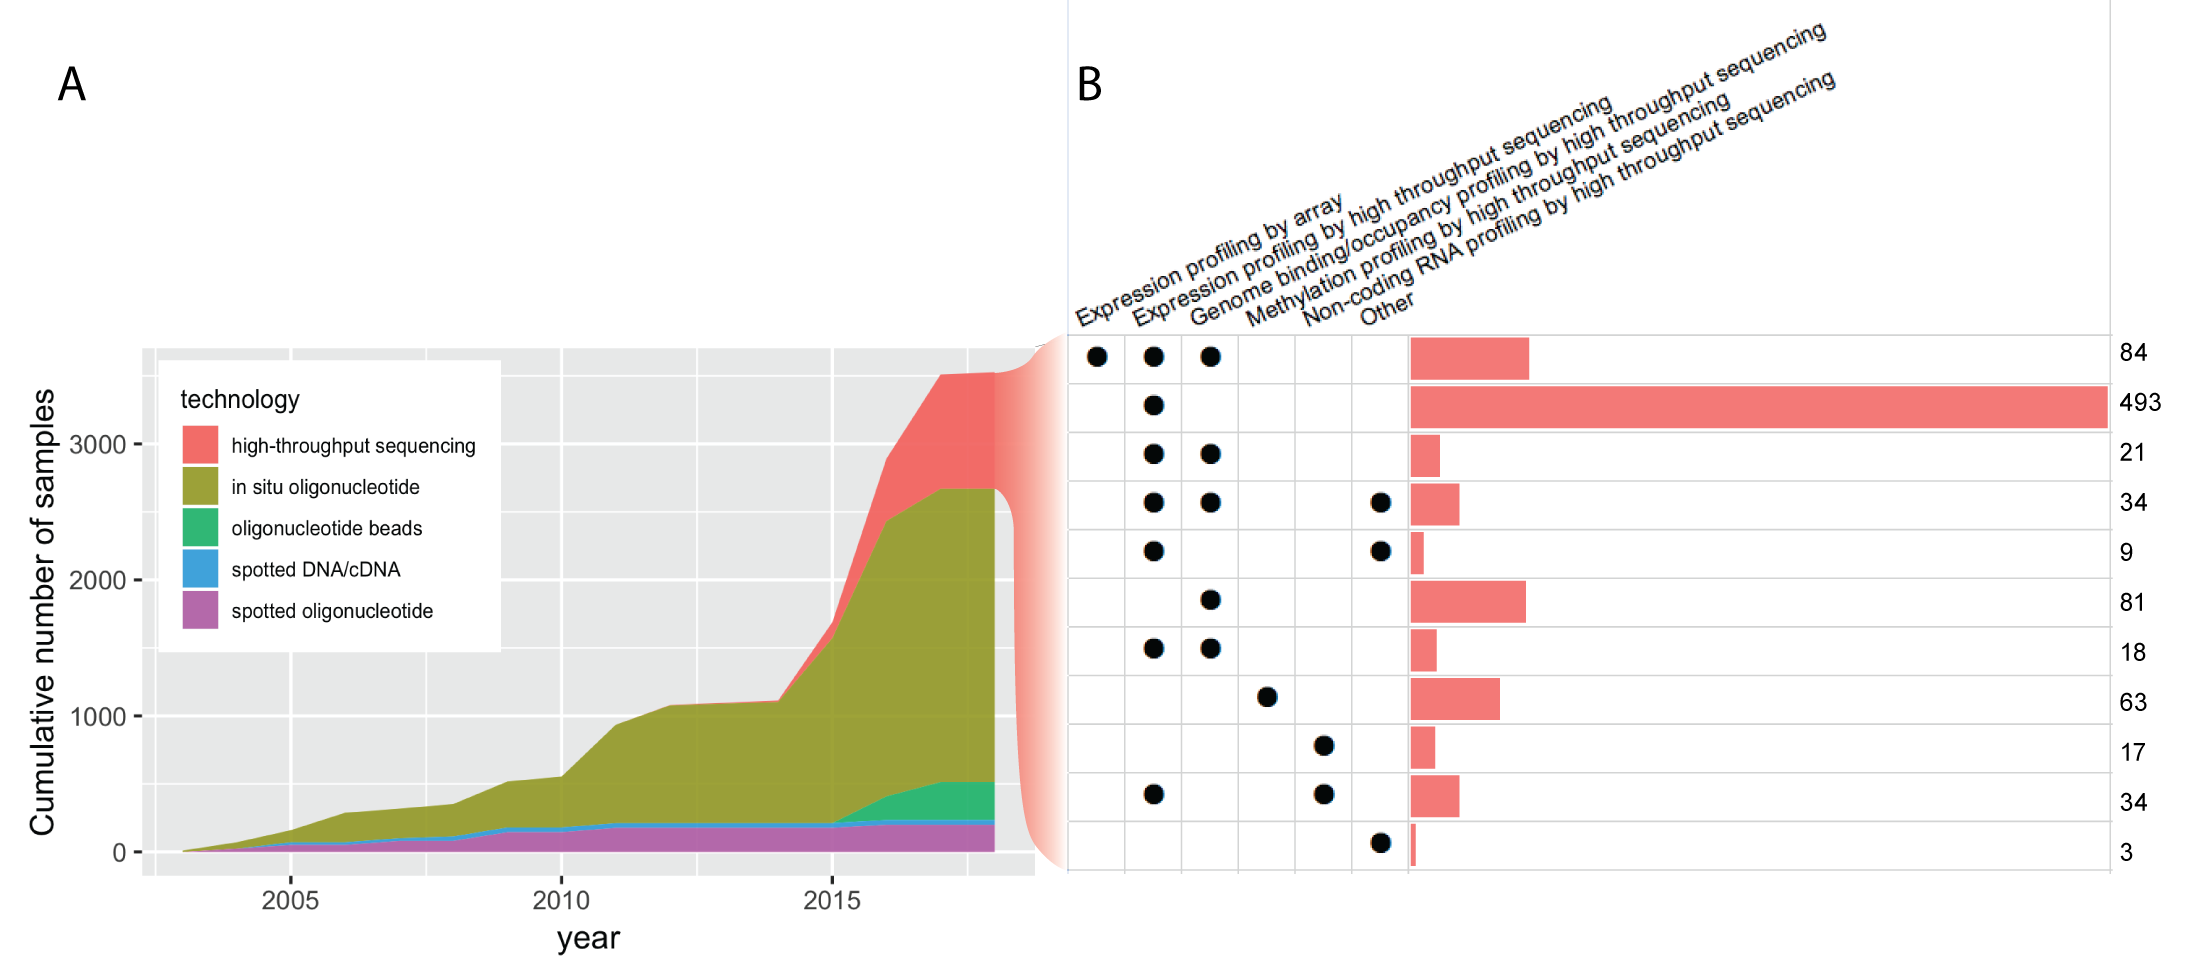
\includegraphics[width=1\linewidth]{assay-count-cardio}
		\caption{(\textbf{A}) The cumulative number of molecular assays (i.e. unique combinations of biosample, study and platform) deposited in GEO by cardiovascular research. (\textbf{B}) Breakdown of high-throughput sequencing assays by the type of study. Expression profiling by high-throughput sequencing, i.e. mRNA-seq assays, are often coupled with another profiling technique, for example, to provide functional read-out of transcription factor binding profiled by ChIP-seq. \label{fig:geo-assay}\\ Note that to avoid excessive over-counting of irrelevant samples such as those from plants or unrelated model organisms, we only counted samples deposited with a PubMed ID pointing to a cardiovascular study. Surveys were done on the GEOmetadb database \citep{Zhu:2008:GEOmetadb} updated on 2018/11/17.}
	\end{figure*} 
	
    While the issues above are generic for all types of research aiming to re-use public data, CVD research benefits from even more abundant sources of biomedical data and faces bigger challenges. Being dominant in biomedical research are genotype-phenotype data in which variations are assayed on pre-defined arrays of SNPs while phenotype is usually recorded as a binary trait, i.e. control vs. disease state. This type of data has enabled the discovery of more than 80,000 variation-phenotype associations by means of genome-wide association studies (GWAS). When deeper phenotype data, such as blood lipid tests and diagnosis (ICD) codes are available, phenome-wide association studies (PheWAS) can be done \citep{Denny:2013:Systematic}. This phenotype data is especially rich in electronic health records (EHRs) abundant at clinical care institutions, enabling powerful analyses when coupled with omics data, as discussed by \cite{Denaxas:2015:Big, Wu:2017:Omic} and exemplified by \cite{Dewey:2016:Distribution,Li:2018:Decoding}. However, EHR data is often unstructured and requires substantial pre-processing to become useful for research purposes, imposing great challenges for data harmonization.
    
    	\begin{figure*}[!tpb]
	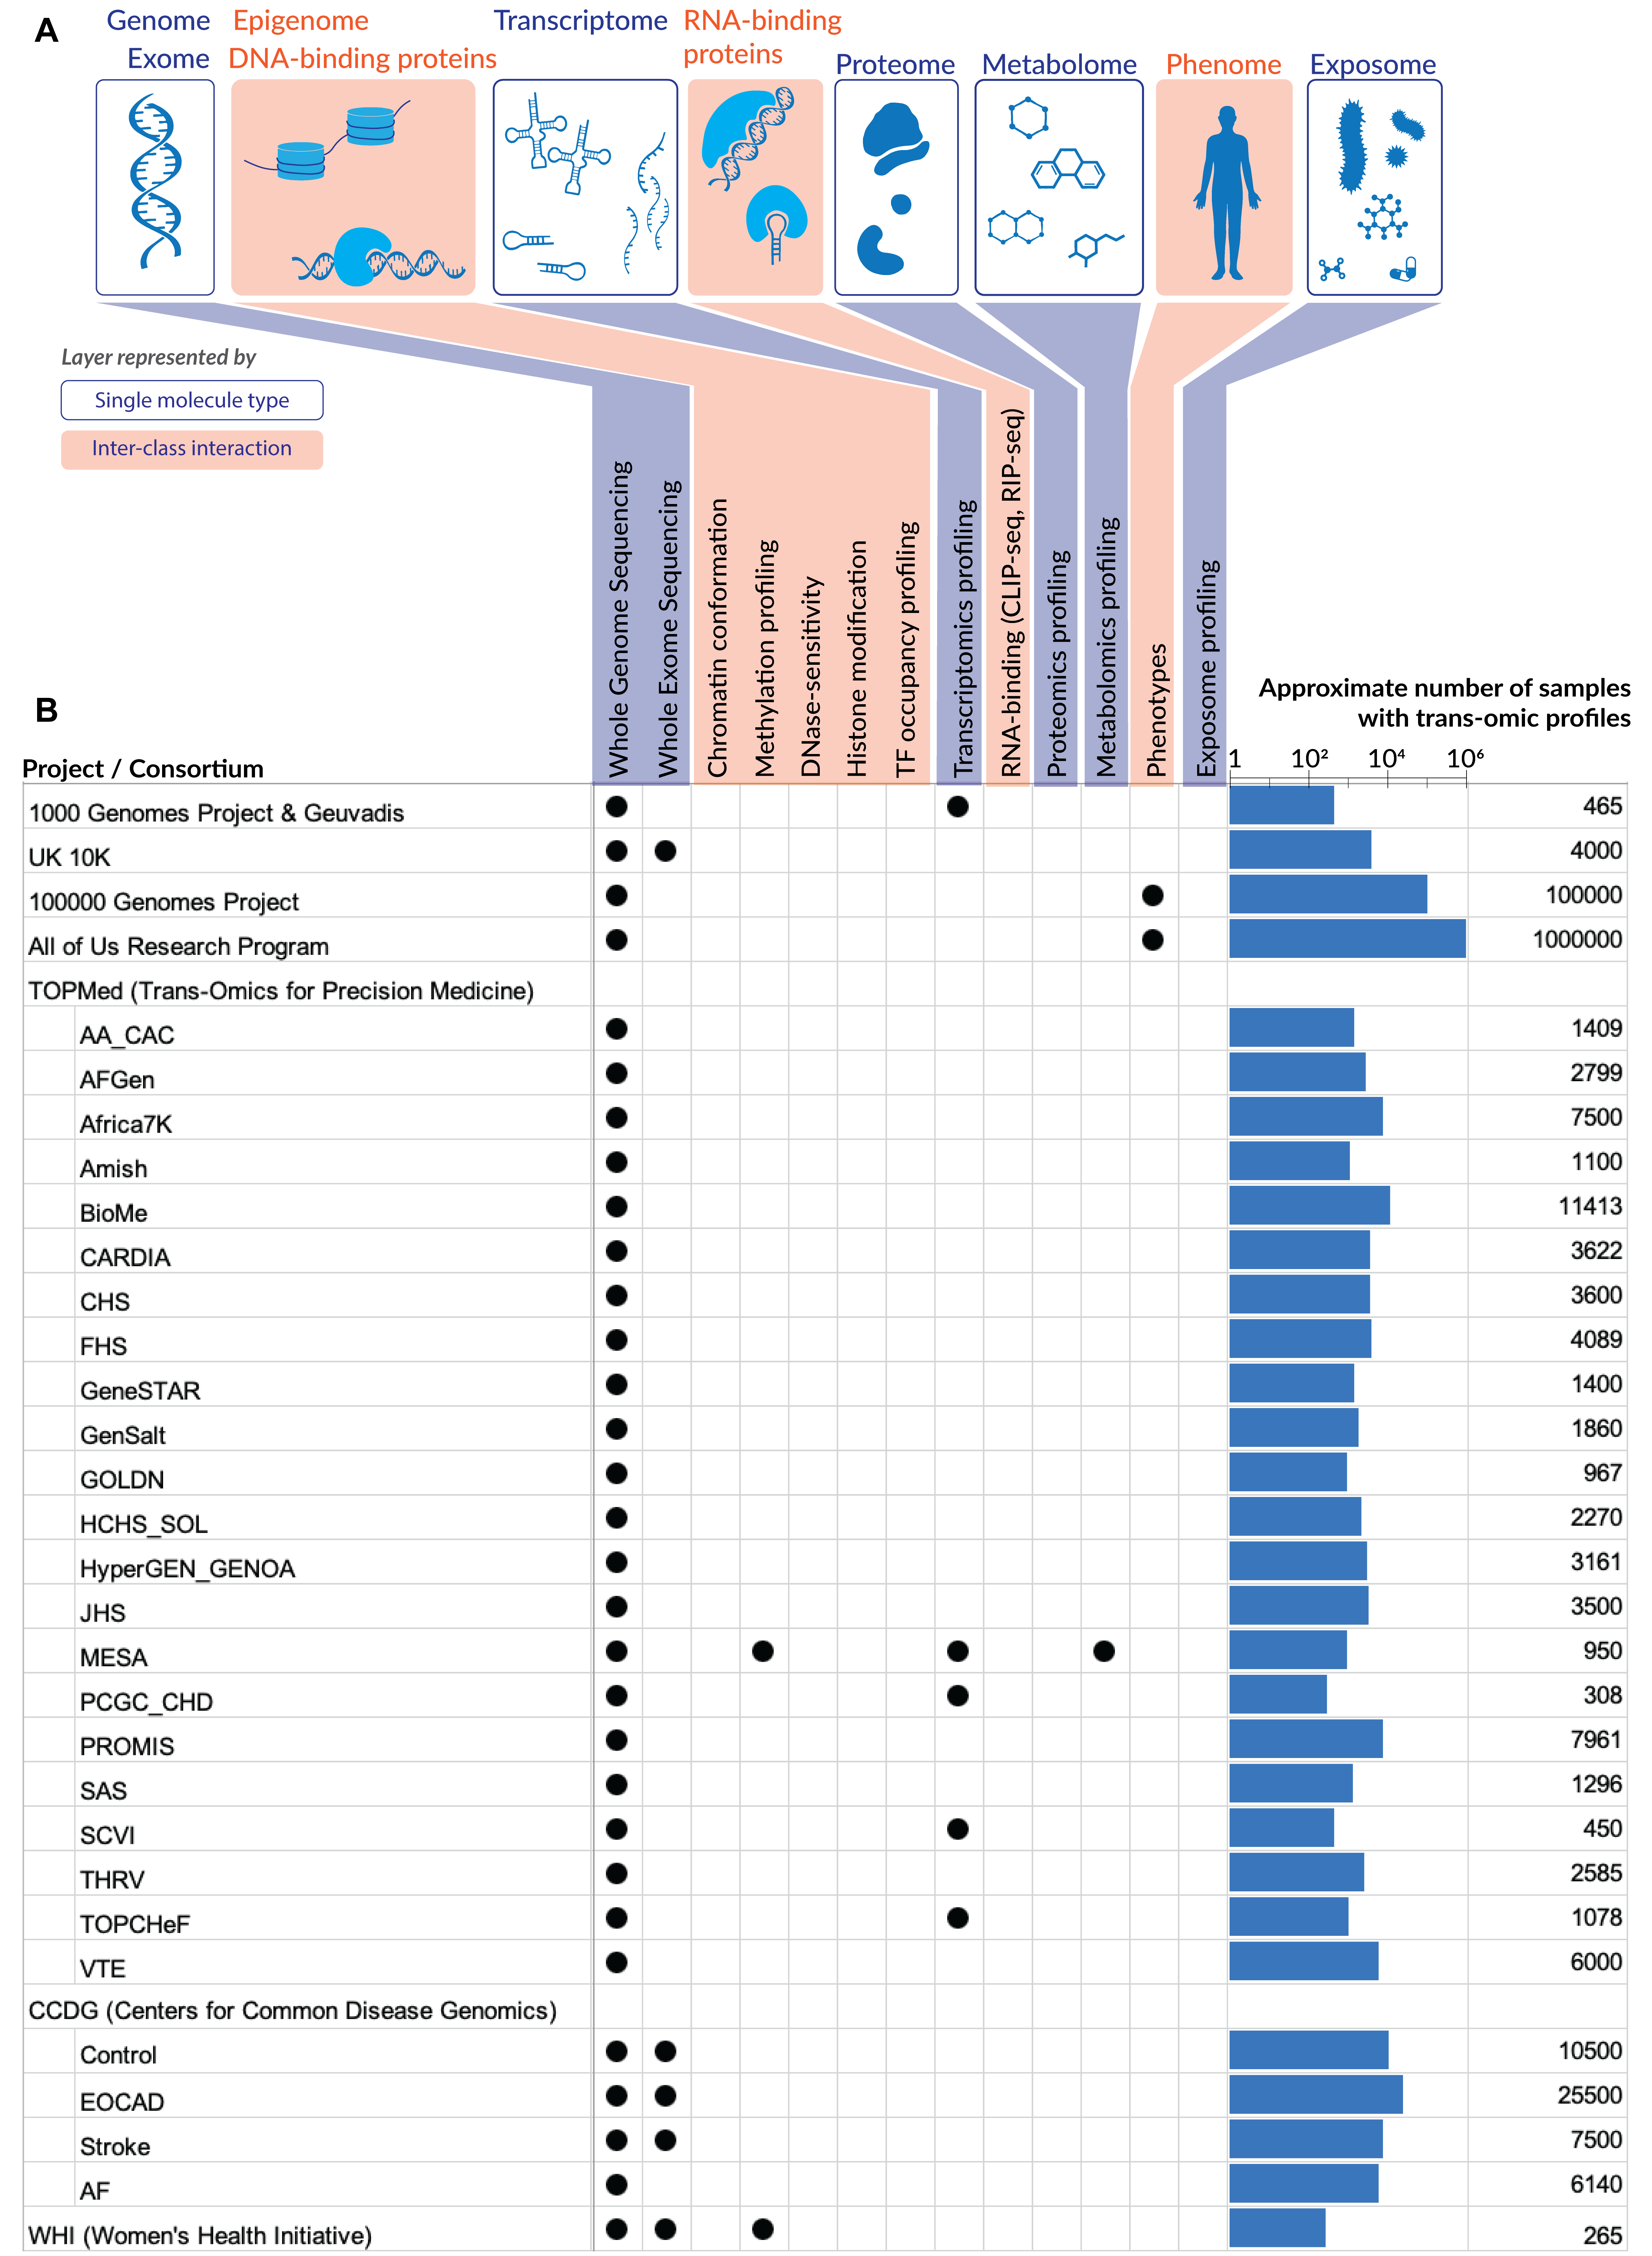
\includegraphics[width=1\linewidth]{trans-omics-data-sets.png}
		\caption{Large omics datasets that are or will be available for CVD research, spanning all major classes of biomolecules: DNA, RNA, proteins and their interactions. For each dataset, the number of samples being assayed across multiple omics are indicated on the right. This number is often smaller than the total number of samples/participants in a given project, because not every sample is run on multiple assays. Beyond the genome, omics datasets become highly complicated, due to the variation across tissues and cell types.}
		\label{fig:trans-omics}
	\end{figure*} 
	
	%%% this part now becomes out-of-place. leave it here for reference
	% Other equally extensive but more structured sources of phenotype data are available from large-scale data collection programs such as the Million Veterans Program (MVP) \citep{Gaziano:2016:Million}, the UK Biobank \citep{Collins:2012:Biobank} and many other national biobanks (for a comprehensive list of human genotype-phenotype data, please see the review by \cite{Brookes:2015:Human}).
	
	Besides existing data, new recent research programs have started to put more focus on high-throughput assays that result in a comprehensive cross-section of biological molecules (DNA, RNA and protein) and their interactions.  Figure \ref{fig:trans-omics} highlights the large datasets that are (or will be) available for cardiovascular research. It is clear that assays for DNA sequence, including whole-genome sequencing and whole-exome sequencing, are still dominant among these studies. However, a decent number of multi-omics experiments are planned to be assayed for transcriptome, methylome, and metabolome, as in the MESA study. The availability of these datasets, especially at the individual-level, is critical to correlate the variations across multiple omics and bridge the gaps from genotype to phenotype.  In general, the analysis of these trans-omics datasets is a fascinating problem -- although the computational approaches envisioned from the early days of gene expression profiling, i.e. differential gene expression analysis, co-expression analysis and gene clustering with subsequent identification of enriched biological pathways \citep{Claverie:1999:Computational} can still bring fruitful analysis \citep{Santolini:2018:personalized}, cardioinformatics is steering towards the integration of multiple omics layers. To this end, the potential of data integration has been recognized as early as a decade ago \cite{Hawkins:2010:Nextgeneration}, leading to the development of many data integration strategies \citep{Ritchie:2015:Methods}. Successful data integration, for example of gene expression and summary-level associations of SNP and phenotypes from GWAS studies, has emerged only recently in CVD research \citep{Gusev:2016:Integrative}. Such approaches, usually referred to as transcriptome-wide association studies (TWAS), are now adopted more widely \citep{Klarin:2018:Genetics}.  Historically, although the first draft of the human genome project had brought a lot of hope and excitement about potential advancements in the diagnosis and treatment of cardiac diseases, such as the ability to identify disease genes within the associated loci, to improve risk estimation based on more precise genotypes, or to personalize the prediction of drug effects on a patient \citep{Komajda:2001:heart}, it seems that a collection of the first "drafts" of the whole "multi-ome" will be required for gaining a deeper understanding of the phenotypic manifestations of CVD across different race/ethnic groups.  All in all, the ability to combine data from every omics layer depicted in Figure \ref{fig:trans-omics}, either at the summary-level or the individual-level, opens up ample directions for cardioinformatics to expand and augment the understanding of cardiovascular disease etiology.
	
	
	\subsection*{Augmented intelligence to advance cardiology}
	In an era of big data and seemingly imperative adoption of machine learning methodologies, the role of human experts turns out to be even more indispensable. Among tasks that still require considerable human judgment include understanding free text data and recognizing visual patterns. 
	% CONSIDER MOVING THIS UP IN THE INTRO
	% As with other areas, cardiovascular research requires expert level domain knowledge to make the best use of machine learning applications, for instance for labeling CVD data or harmonizing it across epidemiological study cohorts.  Without a doubt, domain expertise in cardiology is by no means a tractable problem at scale, exemplified by the insurmountable pile of cardiovascular publications accumulating over the years (Figure \ref{fig:figure1}B). 
	With active research in text-mining and natural language processing, the aim is to liberate human researchers from the time-consuming tasks of reading and making sense of free texts in metadata and documents at scale, including tables, figures, and charts. Since different subdomains in biomedical literature vary along many linguistic dimensions, making text mining systems that perform well on one subdomain not guaranteed to perform well on another \citep{Lippincott:2011:Exploring, Kilicoglu:2018:Biomedical, Khomtchouk:2018:Biochat}, we believe that development of cardioNLP algorithms and dedicated large-scale labeled CVD training datasets will be essential for progress in tasks such as harmonized patient-data meta analyses in cardiovascular precision medicine.
	Recognition of visual patterns, on the other hand, remains a powerful human faculty that needs to be fully exploited rather than replaced. With visualization techniques blossoming across diverse biological data types \citep{Pavlopoulos:2015:Visualizing}, it will be an exciting challenge for cardioinformatic researchers to leverage them for an integrative representation of heterogeneous data layers towards extracting deeper CVD insights. In addition, visualization of many experimental assays and biological processes remains significant challenges, such as visualizing alternative splicing events \citep{Katz:2015:Quantitative,Strobelt:2016:Vials} or large interactive matrices for chromatin conformation data from Hi-C experiments \citep{Kerpedjiev:2018:HiGlass,Lekschas:2018:HiPiler}. In the clinical setting, gearing toward precision medicine entails the requirement of providing more comprehensive data, in a more comprehensible manner to assist clinicans. To this end, visualization and design are critical in improving clinical decision support systems.

	% Search engine and knowledge synthesis \citep{Lutjohann:2011:Sciencenet}. A universal element of all research, knowledge synthesis is under-rated research task. Like most other areas, most of the work in knowledge synthesis has been and has to be done manually in cardiovascular research. Cardiovascular diseases impose the challenge of understanding complex systems of multiple dimensions, creating the pressing need of summarizing and synthesizing knowledge from the vast body of research in a more robust manner.
		
	
	
	%Guidelines, protocol
	%Data visibility
	%efforts to standardize data management and sharing
	%
	
	%\subsection*{Perspectives -- past and present}
	

	
	%* proteomics + transcriptomics \citep{Uhlen:2015:Tissuebased}
	%
	%* genomics + transcriptomics \citep{Klarin:2017:Genetic}

	
	

	%In clinical application, the focus is on facilitating clinical decisions.
	
	%Visualization of chromatin 3D structure emerges as a demand to analyze and present experimental data from conformation capture experiments. The challenges posed by these experiments, being new, high-throughput and  3-dimensional, are actively researched visualization problems \citep{Goodstadt:2017:Challenges}. As a researcher in cardiovascular disease, it is important to stay abreast with the developments in this field to make the most use of the available data.
	
	
	

	
	%%%%%% perspective


	
	%\subsection{Prospective development}
	
	%nanopore sequencing
	
	%single cell
	
	\section*{Closing remarks}
	As we further our quest to understand the genetics and molecular biology of heart disease, many complex clinical indications have become too complicated for traditional approaches. Reflecting on the current body of knowledge, we recognize that many aspects of this complexity can be addressed with more and improved computational methods, as has been the case for bioinformatics in cancer genomics.  But bioinformatics is more than just a powerful toolkit of techniques for conducting high-end cardiovascular disease research, as many important perspectives have arisen from the application, development, and expansion of advanced computational methodologies in this area.  In this review, we discussed some of the important work happening at the multidisciplinary interface of bioinformatics and cardiology, and advocated for shining a brighter spotlight on cardioinformatics as an emerging field, in its own right.  We suggested some future insights based on our understanding of historical perspectives and ongoing work in current CVD research, and we welcome feedback and ideas from the broader scientific community.

	
	\section*{Notes section}
	
	%Common data model: Observational Medical Outcomes Partnership [OMOP] CDM by OHDSI
	
	Outstanding problems
	
	Variant calling and pathogenicity prediction. Currently inconsistent. Mostly developed for protein-coding fraction of the genome (SIFT, Polyphen, etc.), largely ignore the noncoding regions.
	Pathogenicity assignment: variable, conflicting, not applicable for all populations.
	
	Risk estimation
	
	Lack of mechanistic understanding
	
	%{https://www.ncbi.nlm.nih.gov/mesh/68002318} 
	


	
	

	\enlargethispage{12pt}
	
	
	
	
	\section*{Acknowledgements}
	
	BBK acknowledges and thanks the American Heart Association (AHA) for financial support through the AHA Postdoctoral Fellowship program.
	\vspace*{-12pt}
	
	\section*{Funding}
	
	This work has been supported by the American Heart Association (AHA) Postdoctoral Fellowship grant \#18POST34030375 (Khomtchouk).\vspace*{-12pt}
	
	\section*{Competing interests}
	
	BBK is a co-founder of Quiltomics, and Research Associate at the VA Palo Alto Health Care System (Million Veterans Program).  OG is a co-founder of EpiCypher, Inc. and Athelas Therapeutics, Inc.  TLA is Associate Director, Epidemiology Research and Information 
    Center for Genomics, Palo Alto VA Hospital.  The other authors report no conflicts.\vspace*{-12pt} 
	
	\bibliographystyle{natbib}
	%\bibliographystyle{achemnat}
	%\bibliographystyle{plainnat}
	%\bibliographystyle{abbrv}
	%
	%\bibliographystyle{plain}
	%
	\bibliography{cardio}
	
	
	
\end{document}